\documentclass[a4paper]{book}

\usepackage{alphabeta} 
\usepackage{enumitem} 
\usepackage{mathtools}
\usepackage{amsmath, amssymb} 
\usepackage{amsthm}
\usepackage{cancel} 
\usepackage[margin=0.70in]{geometry} 
\geometry{left=2.3cm,right=2.3cm,top=2.4cm,bottom=2.4cm}	%the p1age geometry as defined, A4=210x297mm
\usepackage{graphicx}
\usepackage{wrapfig}
\usepackage[center]{caption}
\usepackage{textcomp}
\usepackage{tabto}
\usepackage{layout}
\usepackage{bm}
\usepackage{minipage-marginpar}
\usepackage[dvipsnames]{xcolor}
\usepackage{hyperref}
\usepackage{dutchcal}
\usepackage{derivative}
\usepackage{esint}
\usepackage{subcaption}
\usepackage{caption}
\usepackage{fancyhdr}
\usepackage{booktabs}
\usepackage{derivative}
\usepackage{braket}
\usepackage[flushleft]{threeparttable}
%\usepackage[capbesideposition=outside,capbesidesep=quad]{floatrow}
\usepackage{derivative}
\usepackage[thinc]{esdiff}
\usepackage{lipsum}
\usepackage{arydshln}
\usepackage{titlesec}
%\usepackage[style=numeric]{biblatex}


\usepackage[square,numbers,super]{natbib}
\bibliographystyle{abbrvnat}



%%RENEW

\newtheorem{problem}{Άσκηση}
\newtheorem*{solution*}{Λύση}
\newtheorem{definition}{Ορισμός}[subsection]
\newtheorem{properties}{Ιδιότητες}[subsection]
\newtheorem{theorem}{Θεώρημα}[subsection]
\newtheorem{protash}{Πρόταση}[subsection]
\newtheorem{porisma}{Πόρισμα}[subsection]
\newtheorem{lemma}{Λήμμα}[subsection]
\newtheorem*{prooof}{Απόδειξη}
\newtheorem*{notes}{Παρατηρήσεις}
\newtheorem*{note}{Παρατήρηση}
\newtheorem*{app}{Εφαρμογή} 
\newtheorem*{example}{Παράδειγμα}
\newtheorem*{examples}{Παραδείγματα}


\newcommand\numberthis{\addtocounter{equation}{1}\tag{\theequation}}
%\renewcommand{\labelenumi}{\roman{enumi}}
\newcommand{\approxtext}[1]{\ensuremath{\stackrel{\text{#1}}{\approx}}}
\renewcommand{\figurename}{Εικόνα.}
\renewcommand{\tablename}{Πίνακας.}
%\renewcommand\refname{New References Header}
\renewcommand*\contentsname{Περιεχόμενα}
%\DeclareDerivative{\odv}{\mathrm{d}}


\title{Μέτρηση του Χρόνου Ζωής των Μιονίων}
\author{Θωμόπουλος Σπυρίδων, ge19042}

\titleformat{\chapter}[hang]{\normalfont\huge\bfseries\color{black}}{\thechapter}{1cm}{}{}
%
\pagestyle{fancy}
%\fancyhead{}
\fancyfoot{}
\fancyhead[LO,LE]{04 Μέτρηση του Χρόνου Ζωής των Μιονίων}
\fancyfoot[CE,CO]{\thepage}


%\addbibresource{bibliogr.bib}
%\bibliographystyle{dinat}
%\bibliography{bibliogr}


\begin{document}
%\begin{titlepage}




\newcommand{\HRule}{\rule{\linewidth}{0.5mm}}

\includegraphics[width=8cm]{Front_Page/logo1.png}\\[1cm] 
\center 
\quad\\[1.5cm]
\textsl{\Large Εθνικό Μετσόβιο Πολυτεχνείο}\\[0.5cm] 
\textsl{\large Σχολή Εφαρμοσμένων Μαθηματικών και Φυσικών Επιστημών}\\[0.5cm] 
\makeatletter
\HRule \\[0.4cm]
{ \huge \bfseries \@title}\\[0.4cm] 
\HRule \\[1.5cm]
\begin{minipage}{0.4\textwidth}
\begin{flushleft} \large
%\emph{Author:}\\
\@author 
\end{flushleft}
\end{minipage}
~
\begin{minipage}{0.4\textwidth}
\begin{flushright} \large
\emph{Επιβλέπων:} \\
\end{flushright}
\end{minipage}\\[3cm]
\makeatother
%{\large An Assignment submitted for the UoS:}\\[0.5cm]
{\large \emph{Εργατήριο Πυρηνικής Φυσικής \& Στοιχειωδών Σωματιδίων}}\\[0.5cm]
%{\large \today}\\[2cm] 
{\large 04 Δεκεμβρίου, 2022}
\vfill 



\end{titlepage}
%%%%%%%%%%555

\begin{titlepage}

\newcommand{\HRule}{\rule{\linewidth}{0.5mm}}

\includegraphics[width=8cm]{logo1}\\[1cm] 
\center 
\quad\\[1.5cm]
\textsl{\Large Εθνικό Μετσόβιο Πολυτεχνείο}\\[0.5cm] 
\textsl{\large Σχολή Εφαρμοσμένων Μαθηματικών και Φυσικών Επιστημών}\\[0.5cm] 
\makeatletter
\HRule \\[0.4cm]
{ \huge \bfseries \@title}\\[0.4cm] 
\HRule \\[1.5cm]
\begin{minipage}{0.4\textwidth}
\begin{flushleft} \large
%\emph{Author:}\\
\@author 
\end{flushleft}
\end{minipage}
~
\begin{minipage}{0.4\textwidth}
\begin{flushright} \large
%\emph{Επιβλέπων:} \\
\end{flushright}
\end{minipage}\\[3cm]
\makeatother
%{\large An Assignment submitted for the UoS:}\\[0.5cm]
{\large \emph{Εργατήριο Πυρηνικής Φυσικής \& Στοιχειωδών Σωματιδίων}}\\[0.5cm]
%{\large \today}\\[2cm] 
{\large 09 Ιανουαρίου, 2023}
\vfill 

\end{titlepage}
%%%%%%%%%%%%%%%5

\section*{Σκοπός}
	Ο σκοπός της εν λόγω εργαστηριακής άσκησης είναι η μέτρηση του μέσου χρόνου ζωής των κοσμικών μιονίων και ο προσδιορισμός της σταθεράς Fermi.
	
	
\section*{Θεωρητική Εισαγωγή}
	Η κοσμική ακτινοβολία που εισέρχεται στην ατμόσφαιρα της Γης πρόκειται για σωματίδια (e, ακτίνες γ, νετρίνα) υψηλής ενέργειας τα οποία παράγονται από τον Ήλιο, από άλλες πηγές εκτός του ηλιακού συστήματος καθώς και από πηγές εκτός του γαλαξία μας. Καθώς εισέρχονται στην ατμόσφαιρα, αλληλεπιδρούν με τα άτομά της(κυρίως Ο,Ν), δημιουργώντας καταιγισμούς από δευτερεύοντα σωματίδια μεταξύ των οποίων και πιόνια. 
	Τα δευτερεύοντα σωματίδια μπορούν είτε να δημιουργήσουν επιπλέον καταιγισμούς είτε, αν δεν έχουν αρκετή ενέργεια, να διασχίσουν για λίγο την ατμόσφαιρα και εν τέλει να διασπαστούν. 
	
	Εμάς μας ενδιαφέρουν τα πιόνια, διότι αυτά δισπώνται μέσω της ασθενούς αλληλεπίδρασης κατά τις παρακάτω αντιδράσεις
		\begin{align}\label{eq1,2}
			\pi^+\rightarrow& \mu^+\nu\\
			\pi^-\rightarrow& \mu^-\bar{\nu}
		\end{align}
	Στο πείραμά μας θα ανιχνεύσουμε τα μιόνια που παράχθηκαν από αυτές, χωρίς να μπορούμε να ξεχωρίσουμε αν πρόκειται για το σωματίδιο $\mu^-$ ή το αντισωματίδιο $\mu^+$.
%	Η αρχική κινητική τους ενέργεια όταν παράγονται στα ανώτερα στρώματα της ατμόσφαιρας είναι περίπου 4GeV. Αυτό σημαίνει ότι η ταχύτητά του θα είναι 
%		\begin{align*}
%			K =& (\gamma-1)m_0c^2 \Rightarrow\\
%		\gamma=& \frac{K}{m_0c^2}+1   = 38.8572\xRightarrow{\text{$m_\mu\simeq 105.66MeV/c^2$}}  \\
%		\beta =& 0.9993
%		\end{align*}
	 Η αρχική κινητική τους ενέργεια όταν παράγονται στα ανώτερα στρώματα της ατμόσφαιαρς $(~15km)$ είναι περίπου 6GeV.
	 Αν δεν λάβουμε υπόψιν μας την θεωρία της Σχετικότητας, τότε τα $\tau=50\mu sec$ που είναι ο χρόνος που απαιτείται για φτάσουν στην επιφάνεια της θάλασσας είναι μεγαλύτερος από τον χρόνο ζωής τους. Λογικά προκύπτει ότι δεν προλαβαίνουν να διανύσουν όλη την απόσταση των 15km, άρα δεν θα έπρεπε να τα ανιχνεύουμε. 
	 Συνεπώς, η ανίχνευσή τους αποτελεί φαινόμενο που υπάγεται στην Ειδική Θεωρία της Σχετικότητας.
	%Άρα, αν δεν λαμβάναμε υπ' όψιν την θεωρία της σχετικότητας τότε θα προέκυπτε πως τα μιόνια δεν θα προλάβαιναν να φτάσουν στην επιφάνεια της θάλασσας καθώς για χρόνο ζωής $\tau\simeq50\mu s $ θα προλάβαιναν να διανύσουν $\Delta x = \beta *c *\tau$
	
	Ο πληθυσμός ενός συνόλου αρχικων μιονίων Ν μειώνεται εκθετικά με τον χρόνο σύμφωνα με την σχέση 
	\begin{align*}\label{eq3}
		N(t) = N_0 e^{-\lambda t} \numberthis
	\end{align*}
	όπου  λ, η σταθερά διάσπασης που συνδέεται με τον μέσο χρόνο ζωής από την σχέση $\tau=1/\lambda$.
	Ο αριθμός $N_0$ και κατ' επέκταση ο N, δεν  αντιστοιχεί στον αρχικό αριθμό μιονίων που υπάρχουν εντός του ανιχνευτή μας αφού κάτι τέτοιο δεν έχει νόημα δεδομένου ότι τα μιόνια εισέρχονται συνεχώς σε αυτόν και διασπώνται.
	 Γι' αυτό θα πρέπει να ορίσουμε ένα νέο μέγεθος το οποίο θα είναι πιό συνεπές με την φύση του πειράματός μας.
	  Συγκεκριμένα αυτό το μέγεθος είναι η κατανομή του χρόνου διάσπασης D(t), όπου η ποσότητα $D(t)\cdot dt$ εκφράζει την πιθανότητα να πραγματοποιηθεί μία διάσπαση σε χρονικό διάστημα dt. Το μέρος των "αρχικών" μιονίων που δισπάτει σε dt δίνεται από τον λόγο $dN/N_0$, άρα παραγωγίζοντας την σχέση (\ref{eq3}) παίρνουμε το D(t)
	\begin{align*}\label{eq4}
		D(t) = \lambda e^{-\lambda t} \numberthis
	\end{align*}	
Οι διασπάσεις του μιονίου οφείλονται στην ηλεκτρασθενή δύναμη και μπορεί να είναι οι παρακάτω 
	\begin{align}\label{eq5}
		\mu^- \rightarrow& e   + \nu_e + \bar{\nu_\mu} \\ 
		\mu^+ \rightarrow& e^+ + \bar{nu_e} + \nu_\mu 
	\end{align}
	
	
	Το κύριο μέρος του ανιχνευτή όπου και παράγονται τα ανιχνεύσιμα σήματα είναι ένας κυλινδρικός πλαστικός σπινθηριστής με διάμετρο 15cm και ύψος 12.5cm. 
	Τα μιόνια, που είναι φορτισμένα, καθώς περνούν από το εσωτερικό του σπινθηριστή ιονίζουν και διεγείρουν τα άτομά του. Αυτό έχει ως αποτέλεσμα την εκπομπή φωτονίου κατά την αποδιέγερσή τους. 
	Τα μιόνια που μας ενδιαφέρουν είναι αυτά που έχουν κινητική ενέργεια έως 160MeV τα οποία δεν προλαβαίνουν να φύγουν εκτός του όγκου του ανιχνευτή και σταματούν εντός του. 
	Αυτά καθώς επιβραδύνονται προκαλούν την εκπομπή φωτονίων από τον σπινθηριστή τα οποία στην συνέχεια οδηγούνται στον πολλαπλασιαστή όπου ενισχύεται το σήμα που παράγουν. 
	Όταν τώρα ένα μιόνιο σταμτήσει, μετά από χρόνο $\tau$, θα δισπαστεί σύμφωνα με τις αντιδράεσις (\ref{eq5}),(6). Επειδή τώρα τα προϊόντα είναι μικρότερης μάζας, θα έχουν αρκετά υψηλή κινητική ενέργεια, με αποτέλεσμα να προκληθούν επιπλέον σπιθηρισμοί από τα $e/e^+$. Τα φωτόνια που δημιουργούνται ανιχνεύονται επίσης από τον φωτοπολλαπλασιαστή μας ο οποίος ενισχύει πάλι το σήμα τους. 
	
	Όταν ανιχνεύεται το πρώτο σήμα από τον φωτοπολλαπλασιαστή, τότε ξεκινά ένα χρονόμετρο που σταματά όταν ανιχνεύσει και το δεύτερο σήμα. Έτσι, το χρονικό διάστημα στο οποίο λειτουργεί το χρονόμετρο μπορούμε να πούμε πως αντιστοιχεί στον χρόνο διάσπασης του μιονίου.
	
	Ακόμη, υπάρχει μία διαφορά μεταξύ των $\mu^- \& \mu^+$. Τα θετικά όταν σταματήσουν απλώς διασπώνται όπως περιγράφηκε παραπάνω.
	Αντιθέτως, τα αρνητικά μπορούν να δεσμευτούν από τα άτομα που έχουν ιονίσει και να σχηματίσουν μιονικά άτομα. Όμως, επειδή έχει πολύ μεγάλη μάζα, το δεσμευμένο μιόνιο θα βρίσκεται πιό κοντα στον πυρήνα και γι' αυτό ενδέχεται να αλληλεπιδράσει με τα πρωτόνιά του κατά την αντίδραση $p+ \mu^-\rightarrow n+\nu_\mu$.
	Η πιθανότητα να συμβεί το παραπάνω φαινόμενο αυξάνεται καθώς αυξάνεται ο ατομικός αριθμός του ατόμου του υλικού καθώς τότε η ηλεκτρική δύναμη που ασκεί ο πυρήνας είναι μεγαλύτερη. Συγκεκριμένα αυτή η πιθανότητα αυξάνει ανάλογα με το $Z^4$. 	
	Εμείς, θέλουμε να μειώσουμε όσο γίνεται την παραπάνω εναλλακτική, διότι τότε ο χρόνος ζωής των αρνητικών μιονίων θα είναι λίγο μικρότερος καθώς θα πραγματοποιείται η παραπάνω αντίδραση. 
	Γι' αυτό επιλέγουμε σπινθηριστή ο οποίος αποτελείται από άτομα μικρού ατομικού αριθμού Z και στην περίπτωσή μας κυρίως από άνθρακα στον οποίο ο χρόνος ζωής των μιονίων είναι $\tau_c = 2.043\pm0.003 \mu s$.
	
	Άρα η μέτρηση του χρόνου ζωής, δεδομένου ότι δεν μπορούμε να ξεχωρίσουμε τα θετικά από τα αρνητικά μιόνια, είναι η μέση τιμή των θετικών και των αρνητικών.
	Οι αντίστοιχες σταθερές διάσπασης (όπως και ο αριθμός των διασπώμενων μιονίων) είναι διαφορετικές για τα δύο σωματίδια και έχουν μέση τιμή 
	\begin{align*}\label{eq7}
		\braket{\lambda} =& \frac{\sum_i \lambda_iN_i}{\sum_i N_i} \Rightarrow\\
		                =& \frac{N^+\lambda^+ + N^- \lambda^-}{N^+ + N^-} \numberthis
	\end{align*}
	
	Άρα για τον μέσο χρόνο ζωής 
		\begin{align*}\label{eq8}
			\tau =& \frac{1}{\braket{\lambda}} \xRightarrow{r = N^+/N^-}\\
			     =& \left( \frac{r \lambda^+ + \lambda^-}{1+r}\right)\Rightarrow^{-1}\\
			     =& (1+r) \left(\frac{1}{\tau^-}+ \frac{r}{\tau^+}\right)^{-1} \\
			     =& (1+r) \left(\frac{\tau^+\tau^-}{\tau^++r\tau^-}\right)\numberthis
		\end{align*}
		
		Επειδή το υλικό του σπινθηριστή είναι οργανικό, δηλαδή αποτελείται κατά μεγάλο μέρος από άνθρακα, μπορούμε να θεωρήσουμε ότι $\tau_-=\tau_c$ και δεδομένου ότι τα θετικά μιόνια δεν επηρεάζονται από το φαινόμενο δέσμευσης από τα άτομα μπορούμε να πούμε αντίστοιχα πως ούτε ο χρόνος ζωής τους επηρεάζεται και πως ισούται με τον χρόνο διπασπασης στο κενό $\tau^+= \tau_0$.
		Για να υπολογίσουμε τον λόγο των πληθυσμών θετικών και αρνητικών μιονίων, μπορούμε να λύσουμε την (\ref{eq8}) προς r 
		\begin{align*}\label{eq9}
			r =- \frac{\tau^+}{\tau^-}\left( \frac{\tau^- -\tau}{\tau^+ - \tau}\right)\numberthis
		\end{align*}
	% Μερικά, δεν ιονίζουν τα άτομα του σπινθηριστή αλλά καθώς εισέρχονται επιβραδύνονται και εκπέμπουν ένα φωτόνιo Bremsstrahlung. 
	
	Τέλος, επειδή τα μιόνια διασπώνται εξαιτίας της ασθενούς αλληλεπίδρασης, μπορούμε να υπολογίσουμε την σταθερά Fermi που σχετίζεται με την ένταση της ασθενούς αλληλεπίδρασης, μέσω του χρόνου διάσπασης των μιονίων 
	\begin{align*}\label{eq10}
		\tau = \frac{192\pi^3\hbar^7}{G_F ^2m^5c^4} \numberthis
	\end{align*}
	
\section*{Πειραματική Διάταξη}


	Η πειραματική μας διάταξη αποτελείται από 
		\begin{itemize}
			\item[.] Σπινθηριστή, ο οποίος είναι τοποθετημένος στο μισό μέρος ενός φωτομονωμένου κυλίνδρου αλουμινίου
			\item[.] Φωτοπολλαπλασιαστή, ο οποίος ενισχύει το σήμα των παραγόμενων από τον σπινθηριστή φωτονίων
			\item[.] Κουτί ηλεκτρονικών και Η/Υ ο οποίος λαμβάνει και επεξεργάζεται τις μετρήσεις
		\end{itemize}
		
	Ο σπινθηριστής ιονίζεται από φορτισμένα ηλεκτρόνια, μιόνια, αλλά και από φωτόνια. Συνεπώς τα σήματα που λαμβάνουμε δεν προέρχονται μόνο από μιόνια. Για να περιορίσουμε τα παραπάνω φαινόμενα υποβάθρου, μπορούμε να κρατάμε μόνο τα γεγονότα που απέχουν χρονικό διάστημα περίπου ίσο με αυτό που αναμένουμε και επίσης, μπορούμε να εκτιμήσουμε το μέγεθος του υποβάθρου από τις περιοχές μεγάλου χρόνου όπου δεν θα υπάρχουν πραγματικά γεγονότα.
	
	
\section*{Πειραματική Διαδικασία - Επεξεργασία Μετρήσεων}
	\subsection*{Υπολογισμός Χρόνου Ζωής}
	Αφού συνδέσουμε τον ανιχνευτή με το κουτί ηλεκτρονικών και κατ' επέκταση με τον Η/Υ, ρυθμίζουμε την τάση στα άκρα του ανιχνευτή στα $1000V$, του φωτοπολλαπλασιαστή στα 240mV και... αν ο Η/Υ είναι αρκετά συνεργάσιμος, ξεκινάμε την καταγραφή γεγονότων από το πρόγραμμα.
	
	Τα δεδομένα περιέχονται στο αρχείο \textit{data\_muons}, στην πρώτη στήλη του οποίου καταγράφεται (σε ns) η χρονική διαφορά μεταξύ των δύο σημάτων που λαμβάνει ο ανιχνευτής μας. Αν ο χρόνος είναι $\geq 40\times10^3 ns$ θεωρούμε πως το ενδεχόμενο μιόνιο δεν έχει διασπαστεί και αγνοούμε το αντίστοιχο γεγονός. 
	Τρέχοντας το αρχείο \textit{muons\_fit} προσαρμόζουμε στα δεδομένα μας μία καμπύλη της μορφής 
	\begin{align*}\label{eq11}
		f(t;\tau,A) = Aexp(-t/\tau_{obs}) \numberthis
	\end{align*}
 μέσω της ελαχιστοποίησης της συνάρτησης 
 	\begin{align*}\label{eq12}
 		\chi^2 = \sum_i \frac{(n_i(t_i)-f(t_i))^2}{\sigma_i} \numberthis
 	\end{align*}
 όπου Α,$\tau_{obs}$ είναι οι παράμετροι του μοντέλου μας οι οποίοι προσδιορίζονται από την ελαχιστοποίηση της $\chi^2$, με $\tau_{obs}$ τον χρόνο ζωής του μίονίου,
  $n_i(t_i)$ είναι ο αριθμός των γεγονότων που αντιστοιχούν σε χρόνο διάσπασης $t_i$ και $\sigma_i = \sqrt{n_i}$ είναι το σφάλμα.
 
 Η καμπύλη που προκύπτει φαίνεται στην παρακάτω γραφική παράσταση 
 	\begin{figure}[h!]
 		\centering
 		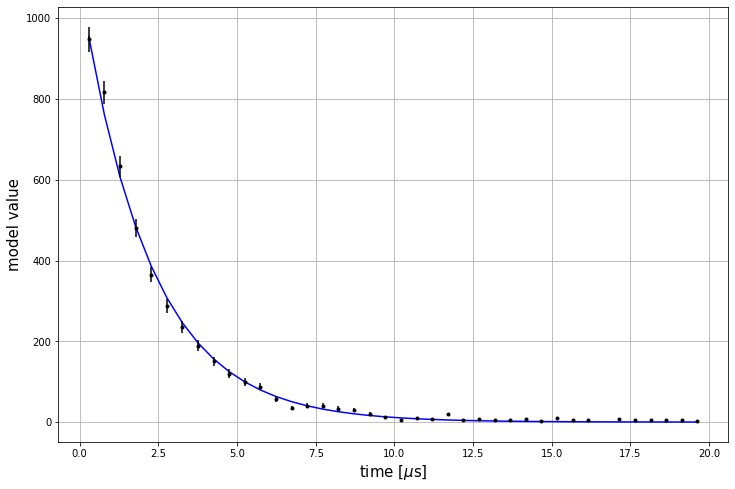
\includegraphics[scale=0.6]{fitted_model.png}
 		\caption{Η καμπύλη $Aexp(-t/\tau_{obs})$ προσαρμοσμένη στα δεδομένα του πειράματος}
 		\label{fig1}
 	\end{figure}
 	

Οι παράμετροι το μοντέλου με τα αντίστοιχα σφάλματά τους προκύπτουν 
	\begin{align*}\label{eq13}
		\tau_{obs} =& (2.19   \pm 0.05  )\mu s  \numberthis
	\end{align*}
\vspace{-0.5cm}
	\begin{align*}\label{eq14}
		A    =& 1088.08 \pm 36.59           \numberthis
	\end{align*}

Η βιβλιογραφική τιμή του χρόνου ζωής των μιονίων είναι $\tau_{bib} = 2.19737\mu s$.
	Παρατηρούμε πως οι δύο τιμές ταυτίζονται απόλυτα μέχρι το δεύτερο δεκαδικό τους ψηφίο, με σχετικό σφάλμα $\sim0.3\%$.
	
	Αν δεν λάβουμε υπ' όψιν την Ειδική Θεωρία της Σχετικότητας και θεωρήσουμε πως ο χρόνος ζωής του μιονίου είναι ίδιος στο σύστημα του εργαστηρίου και του μιονίου, τότε παρατηρούμε πως ο χρόνος ζωής του είναι μικρότερος από τον χρόνο που απαιτείται για να φτάσει στον ανιχνευτή μας από το σημείο που παράγεται στα 15km.
	Συγκεκριμένα, αν θεωρήσουμε πως το μιόνιο έχει ταχύτητα 0.98c, τότε ο χρόνος που απαιτείται για να φτάσει στον ανιχνευτή μας είναι περίπου $t=s/0.98c=15km/c\simeq50\mu s >\tau_{obs}$.
	
	Από τους μετασχηματισμούς του Lorentz προκύπτει πως δύο γεγονότα που απέχουν  χωρικά $\Delta x=0$ σε ένα σύστημα και $\Delta x'\neq0$ σε ένα άλλο, θα συμβαίνουν μεταξύ διαφορετικών χρονικών διαστημάτων που συνδέονται από την σχέση $\Delta t' = \gamma \Delta t$.
	Στο παράδειγμα του μιονίου, το μιόνιο αντιστοιχεί στο άτονο σύστημα, καθώς η διάσπαση στο σύστημά του συμβαίνει σε $\Delta x = 0$, άρα το δικό μας σύστημα αντιστοιχεί στο τονούμενο.
	Γι' αυτό για τον χρόνο ζωής (διάστημα μεταξύ δημιουργίας και διάσπασης) έχουμε 
	$\tau_{\mu}' = \gamma \tau_{\mu}$.
	\footnote{Θεωρούμε πως $\tau_{\mu} = \tau_{obs}$, δηλαδή πως στο πείραμά μας μετράμε τον χρόνο ζωής στο σύστημα του μιονίου. Αυτό διότι στον ανιχνευτή μας το μιόνιο σταματάει προτού ξεκινήσει η διάσπασή του, επομένως τότε το σύστημά του ταυτίζεται με το δικό μας.} 
	
		Για παράδειγμα αν θεωρήσουμε πως θα έχει κινητική ενέργεια $~6GeV$ τότε από την σχέση $T=(\gamma-1)m_\mu c^2$ προκύπτει ο παράγοντας $\gamma\simeq58.14$, άρα στο σύστημα του εργαστηρίου ο χρόνος ζωής του είναι $\tau_\mu' = 58.14\tau_{lab} =  127.33\mu s > \tau_\mu= 2.19\mu s$. Έτσι εξηγείται το γεγονός ότι μπορούμε να ανιχνεύσουμε τα μιόνια.
		
		Αντίστοιχη δικαιολόγηση μπορεί να προκύψει από την συστολή του μήκους.
	Πάλι από μετασχηματισμούς Lorentz προκύπτει ότι το μήκος της διαδρομής του μιονίου όπως το μετράμε εμείς L' και όπως το μετράει το ίδιο το μιόνιο στο σύστημά του L, είναι διαφορετικά και συνδέονται με την σχέση 
	$L' = L/\gamma=15km/58.14 \simeq 258m$. 
	Άρα ο αντίστοιχος χρόνος που απαιτείται για να το διανύσει είναι $L'/0.999c\simeq 0.8\mu s$ που είναι μικρότερο από τον χρόνο ζωής του μιονίου στο σύστημά του.
	
	Ακόμη, μέσω του χρόνου ζωής του μιονίου μπορούμε να υπολογίσουμε την σταθερά σύζευξης Fermi από την σχέση (\ref{eq10}) και το σφάλμα της\footnotemark
	\begin{align*}\label{eq15}
			G_F = (8.99\pm0.10)\times10^{-44}eV\cdot s^3
		\end{align*}	
\footnotetext{Το σφάλμα προκύπτει από διάδοση του σφάλματος του χρόνου ζωής του μιονίου καθώς τα υπόλοιπα μεγέθη έχουν αμελητέο σφάλμα. Από την (\ref{eq10}) έχουμε $G_F=\sqrt{\frac{192\pi^3\hbar^7}{\tau m^5 c^4}}$. Άρα το σφάλμα είναι \\
$\delta G_F=\sqrt{\left(\pdv{G_F}{\tau}\delta\tau\right)^2}= G_F\delta\tau/2\tau\simeq 0.1\times10^{-44}eV\cdot s^3$}
	Ή σε μία λίγο πιό κομψή μορφή γράφεται
	\begin{align*}
		\frac{G_F}{(\hbar c)^3} = (1.17 \pm 0.01) \times10^{-5} GeV^{-2}	
	\end{align*}		
	
	Η βιβλιογραφική τιμή είναι $(G_F/(\hbar c)^3)_{bib} =1.166\times10^{-5}GeV^{-2}$, εξαιρετικά κοντά σε αυτή που βρήκαμε εμείς και στα όρια του σφάλματος, με σχετικό σφάλμα $\sim 0.3\%$.
	
	
	Ακόμη, μπορούμε να υπολογίσουμε την αναμενόμενη τιμή του χρόνου ζωής των μιονίων λαμβάνοντας υπ' οψιν και το φαινόμενο τηε δέσμευσής τους από τα άτομα άνθρακα του σπινθηριστή. Από την σχέση (\ref{eq8}), θεωρώντας $r=1$ (ίσος αριθμός θετικών \& αρνητκών μιονίων), $\tau^- =\tau_c = (2.043\pm0.003)\mu s$ και $\tau^+ = \tau_{bib} = 2.19703\pm0.00004)\mu s$ 
	\begin{align*}%\label{eq16}
      \tau =& (1+r)\left(\frac{\tau^-\tau^+}{\tau^+ + r\tau^-}\right)\Rightarrow\\
	  \tau =& (2.12 \pm 0.01)\mu s \numberthis \footnotemark
	\end{align*}
	
	\footnotetext{Το σφάλμα από διάδοση είναι $\delta \tau_{exp} =\sqrt{\left( \pdv{\tau}{\tau^+}\delta\tau^+\right)^2+\left( \pdv{\tau}{\tau^-}\delta\tau^-\right)^2}=
	 \sqrt{\left(\frac{\tau^2r}{\tau^{+2}}\delta\tau^+\right)^2+ \left( \frac{\tau^2}{\tau^{-2}}\delta\tau^-\right)^2}==
	 \tau^2\sqrt{\left(\frac{r}{\tau^{+2}}\delta\tau^+\right)^2+ \left( \frac{1}{\tau^{-2}}\delta\tau^-\right)^2} =
	  4.49\times10^{-12}\sqrt{69+5\times10^5}\simeq 0.003\mu s\rightarrow0.01\mu s$}
	
	\newpage
	\subsection*{Υπολογισμός Πιθανοτήτων}
	
	Υποθέτουμε ότι η ανίχνευση διασπώμενων μιονίων ανά λεπτό αποτελεί μία τυχαία μεταβλητή η οποία ακολουθεί την κατανομή Poisson 
	\begin{align*}%\label{eq17}
		P(n,t) = \frac{t^n e^{-t}}{n!}\numberthis
	\end{align*}

Άρα η πιθανότητα να μην δούμε ένα μιόνιο σε 1 λεπτό είναι 
	\begin{align*}%\label{eq}
		P(n=0,t=1) = \frac{e^{-1} }{1} = 0.37 
	\end{align*}
Και η πιθανότητα να μην δούμε ένα μιόνιο σε 4 λεπτά είνα 
	\begin{align*}%\label{eq}
		P(n=0,t=4) = \frac{e^{-4}}{1} = 0.018
	\end{align*}
	
	
	
	
\section*{Συμπεράσματα}
	Οι στόχοι του εργαστηρίου επιτεύγχθηκαν και μάλιστα με μεγάλη ακρίβεια. Η σταθερά σύζευξης Fermi, όσο και ο χρόνος ζωής του μιονίου προσδιορίστηκαν με σχετικό σφάλμα $\sim0.3\%$ από την βιλιογραφική τιμή τους. Αυτή η άσκηση μάλλον κερδίζει με διαφορά το βραβείο πιό ακριβούς μέτρησης των εργαστηρίων της ΣΕΜΦΕ. 
\end{document}